\section{Results}

\subsection{Absolute external performance}

The complete external inventory contained \ProbeRuns{} selected checkpoints and
\ExternalPredictions{} subject-level predictions. The final-layer mean-linear
baseline achieved mean Pearson $r=\BaselinePearson{}$, MAE
\BaselineMAE{} years, RMSE \BaselineRMSE{} years, and $R^2=
\BaselineRSquared{}$. Its mean calibration slope was
\BaselineCalibrationSlope{}, indicating that correlation alone did not imply
well-calibrated age estimates.

\begin{table}[t]
  \centering
  \small
  \caption{Mean primary-cohort metrics across ten optimization seeds. MAE and
  RMSE are in years. Calibration parameters are descriptive.}
  \label{tab:absolute-metrics}
  \input{generated/main_metrics}
\end{table}

The rich-statistics residual head had the largest average Pearson among the
tested heads, while the multi-query head had the lowest mean absolute and root
mean-squared errors. These rankings are descriptive: the primary question was
whether paired Pearson gains were stable under the complete decision rule.

\subsection{Paired confirmatory comparisons}

Relative to the matched baseline, mean Pearson increased by
\LayerLinearPearsonDelta{} for the penultimate-layer linear probe,
\RichResidualPearsonDelta{} for the rich-statistics residual head, and
\MultiQueryPearsonDelta{} for the multi-query head. All three Holm-adjusted
one-sided $p$-values were below the predeclared threshold. Nevertheless, their
95\% hierarchical-bootstrap intervals extended below zero: the respective
lower bounds were \LayerLinearCILow{}, \RichResidualCILow{}, and
\MultiQueryCILow{}. Thus none satisfied every required condition.

\begin{table}[t]
  \centering
  \small
  \caption{Paired confirmatory comparisons against the final-layer mean-linear
  baseline. W/T/L denotes wins, ties, and losses across seeds.}
  \label{tab:confirmatory}
  % Generated table; do not edit.
\begin{tabular}{lrrrrrr}
\toprule
Candidate & Mean $\Delta r$ & 95\% CI & Holm $p$ & W/T/L & Worst $\Delta r$ & Stable \\
\midrule
Layer-mixed linear & 0.008 & [-0.019,\ 0.036] & 0.003 & 10/0/0 & 0.004 & no \\
Rich-statistics residual & 0.032 & [-0.050,\ 0.125] & 0.003 & 10/0/0 & 0.025 & no \\
Multi-query rich-statistics & 0.010 & [-0.114,\ 0.154] & 0.004 & 8/0/2 & -0.003 & no \\
\bottomrule
\end{tabular}

\end{table}

\begin{figure}[t]
  \centering
  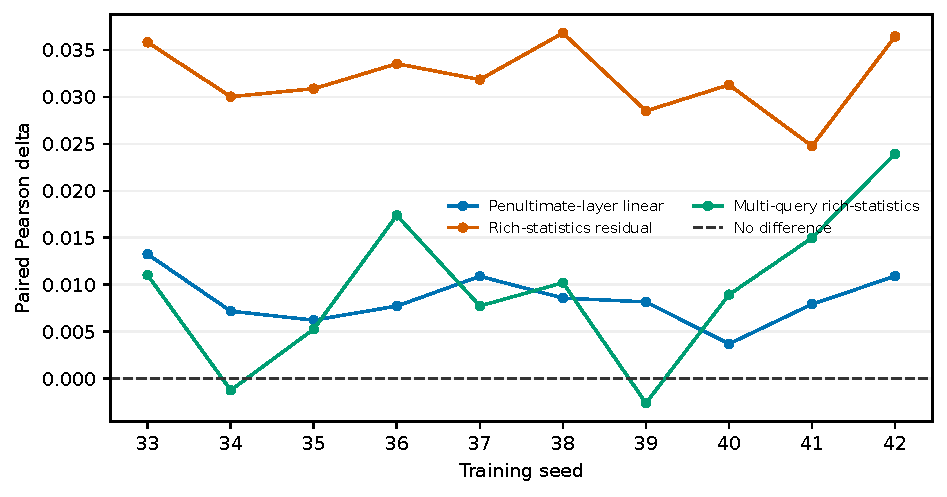
\includegraphics[width=0.93\linewidth]{generated/seed_deltas.pdf}
  \caption{Paired external Pearson differences for each optimization seed.
  Positive values favor the candidate head.}
  \label{fig:seed-deltas}
\end{figure}

The per-seed view shows that layer selection and rich-statistics residualization
were directionally consistent across the observed seeds, whereas the
multi-query model lost on \MultiQueryLosses{} seeds. Directional seed
consistency did not remove uncertainty induced by the finite external cohort,
as visualized by the joint seed-and-subject bootstrap intervals.

\begin{figure}[t]
  \centering
  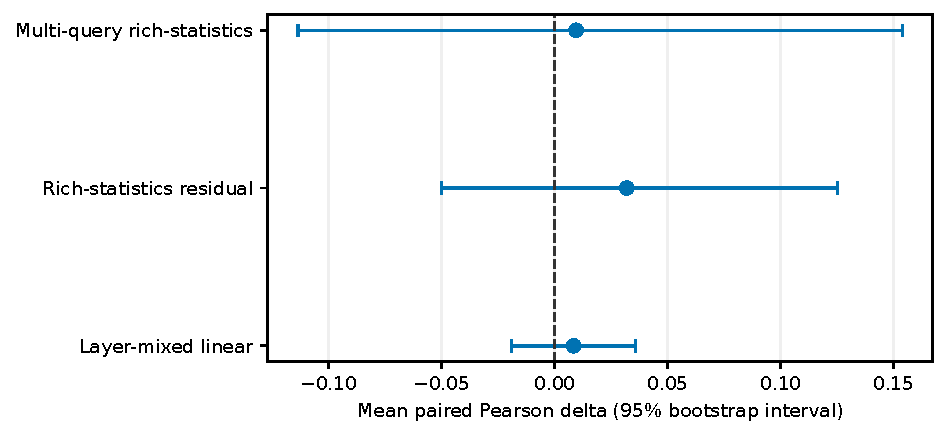
\includegraphics[width=0.90\linewidth]{generated/bootstrap_intervals.pdf}
  \caption{Mean paired Pearson differences and 95\% hierarchical-bootstrap
  intervals. Every interval intersects the no-difference line.}
  \label{fig:bootstrap}
\end{figure}

\subsection{Calibration}

All heads had mean calibration slopes above one, with the multi-query model
closest to the ideal slope among the four. Intercepts were also displaced from
zero. These patterns reinforce that a ranking by correlation is not a complete
assessment of the resulting age predictions.

\begin{figure}[t]
  \centering
  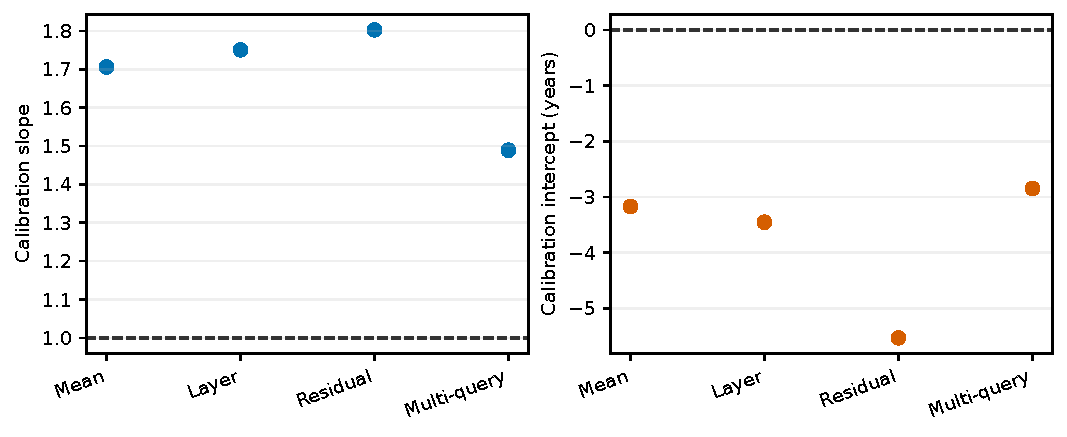
\includegraphics[width=0.92\linewidth]{generated/calibration_summary.pdf}
  \caption{Descriptive mean calibration slopes and intercepts. Dashed lines
  denote the ideal slope of one and intercept of zero.}
  \label{fig:calibration}
\end{figure}
